\UseRawInputEncoding

\textbf{Abstract.} As part of a larger project on argument mining of Swedish parliamentary data, we have created a semantic graph that, together with named entity recognition and resolution (NER), should make it easier to establish connections between arguments in a given debate. The graph is essentially a semantic database that keeps track of Members of Parliament (MPs), in particular their presence in the parliament and activity in debates, but also party affiliation and participation in commissions. The hope is that the Swedish PoliGraph will enable us to perform named entity resolution on debates in the Swedish parliament with a high accuracy, with the aim of determining to whom an argument is directed.

\section{Introduction}

While argument mining still is a young task in the field of computational linguistics, it has received much attention during the last five years. Parliamentary data is not only an ideal application of this, but also often a treasure trove of training data, given its standardised language and detailed accompanying metadata. Debates from the Swedish parliament, which will be the main focus for this project, are available from 1971 until the present date, with particularly detailed metadata present from 1993 and onward. The ultimate task of our project is to evaluate and develop tools for argument mining on these debates. As a first step, we have created the Swedish PoliGraph, a semantic graph to aid us in achieving our goal. Following the completion of this graph, we will use it to improve upon methods for NER that, in turn, can assist in determining the structure of discourse present in the various debates in the Swedish parliament.

\section{About the Swedish Parliamentary Data}

Coinciding with the ratification of \emph{Lag (2010:566) om vidareutnyttjande av handlingar från den offentliga förvaltningen}, a law commonly known as \emph{PSI-lagen} `re-use of Public Sector Information', \emph{Riksdagens öppna data} `parliamentary open data', from here on abbreviated as RÖD) was published in 2010. A massive collection of structured content from the databases of the Swedish parliament, RÖD is continuously updated, both with new data and with the gaps in older data filled in.

The available data is sorted into five categories: Documents, MPs, voting results, speeches and calendar. Of these, the documents constitute the largest category, with a substantial amount of data from 1971 and onward. The categories for MPs and voting results consist mostly of metadata, while speeches are transcripts of both addresses and replies, accompanied by extensive metadata, starting from 1993.\footnote{An exhaustive description of the various available datasets cannot be given in this paper. The documents category in particular contains 40 different types of documents. Please see the RÖD website at \url{https://data.riksdagen.se/} and Riksdagen's page for descriptions of the various document types at \url{https://www.riksdagen.se/sv/Dokument-Lagar/}.}

In addition to their availability through a well documented API, the data can be downloaded in several formats, including HTML, plain text, CSV, XML, JSON and SQL.

For the initial stages of this project, we choose to focus on the speeches category (\emph{anföranden} in Swedish), as this dataset is relatively consistent, fairly complete and contains the most metadata. Once we have developed our methods for argument mining, we can extend the data to include older protocols from debates dating back to 1971. A \emph{speech} in this context refers to an entry in a debate, and the term will be used in this sense throughout the paper.

\section{Development Details}

\subsection{The RÖD Documents}

After removing a small number of ill-formed documents, we ended up with 325\,202 speeches in our dataset. Starting with the downloads from RÖD in JSON format, each speech is one document, and constitutes one entry in a debate in the Swedish parliament. Most debates are on specific propositions from either the government, parliamentarians or commissions, though there are also weekly meetings in the parliament where MPs can address ministers directly with questions. Debates usually end with a voting session, the details of which are stored in a different dataset. At a later stage, we will combine our argument analysis with the votes in order to better understand the relationship between debates and the resulting votes.

\subsection{Speeches}

A typical speech document contains the metadata as outlined in table \ref{poli-anf-table}. Of particular importance here is \emph{dok\_id}, which designates the meeting in question, \emph{anforande\_nummer}, referring to the number of this speech in the chronological order of speeches during that meeting, and \emph{rel\_dok\_id}, which is the ID of the proposition that is being debated. In order to map a single debate, we therefore need to:

\begin{enumerate}
    \item Find all speeches with a given \emph{rel\_dok\_id}.
    \item Determine the meeting(s) this was debated in.
    \item Establish the chronological order of the speeches during these meetings.
    \item Analyse each speech and attempt to determine which previous speech or speeches (if any) was/were addressed or argued against.
\end{enumerate}

\subsection{Members of Parliament}
\label{sec:mp}

For the Swedish PoliGraph, we have combined the speech information with metadata from the MP category, which includes basic biographical information as well as a complete history of their roles in the parliament. Such roles are usually their time working as an MP and commission work, but also longer sick leave is listed here as well as their substitutes in those cases. In addition to the essential identifiers ``name'' and ``party'', mappings are also created to MP's Wikidata-IDs and their listed name there, which sometimes provide more detail than the names as they are stored in RÖD.

The roles of MPs are generally described in terms of positions, where each assignment (or leave from that assignment) is stored as a factual predicate with eight arguments:
\begin{enumerate}
    \item MP-ID\\ \emph{A unique ID for each MP.}
    \item Agency code\\ \emph{An identifying code for the agency. This can be ambiguous, as parties and commissions sometimes use the same identifier.}
    \item Role\\ \emph{The MP's role in the agency, e.g. parliamentarian, commission chair or substitute.}
    \item From\\ \emph{Starting date of the position.}
    \item To\\ \emph{End date of the position.}
    \item Type\\ \emph{The type of position, usually either ``kammaruppdrag'' for the parliament or ``uppdrag'' for commission work.}
    \item Uppdrag\\ \emph{The info here varies. For commission work and other extraparliamentary duties, it contains the full name of the commission or equivalent. For extended leave, it lists the name of substitutes.}
    \item Status\\ \emph{The MP's presence or absence during the given period.}
\end{enumerate}

\begin{table}[t!]
\begin{center}
\begin{tabular}{|l|l|}
\hline \textbf{Property} & \textbf{Description} \\ \hline
dok\_hangar\_id & Internal document ID \\
dok\_id  & Meeting + speech no. \\
dok\_titel & Protocol title \\
dok\_rm & Parliamentary year \\
dok\_nummer & Number of meeting \\
dok\_datum & Date of speech \\
avsnittsrubrik & Topic title \\
underrubrik & Topic subtitle \\
kammaraktivitet & Type of debate \\
anforande\_id & Unique speech ID \\
anforande\_nummer & Speech number in debate \\
talare & Speaker name \\
parti & Speaker party \\
anforandetext & Full speech text \\
intressent\_id & Speaker's ID \\
rel\_dok\_id & Document being debated \\
replik & Speech type \\
systemdatum & Date of publishing \\
\hline
\end{tabular}
\end{center}
\caption{\label{poli-anf-table} A typical speech document. }
\end{table}

\begin{figure*}
 \centering 
 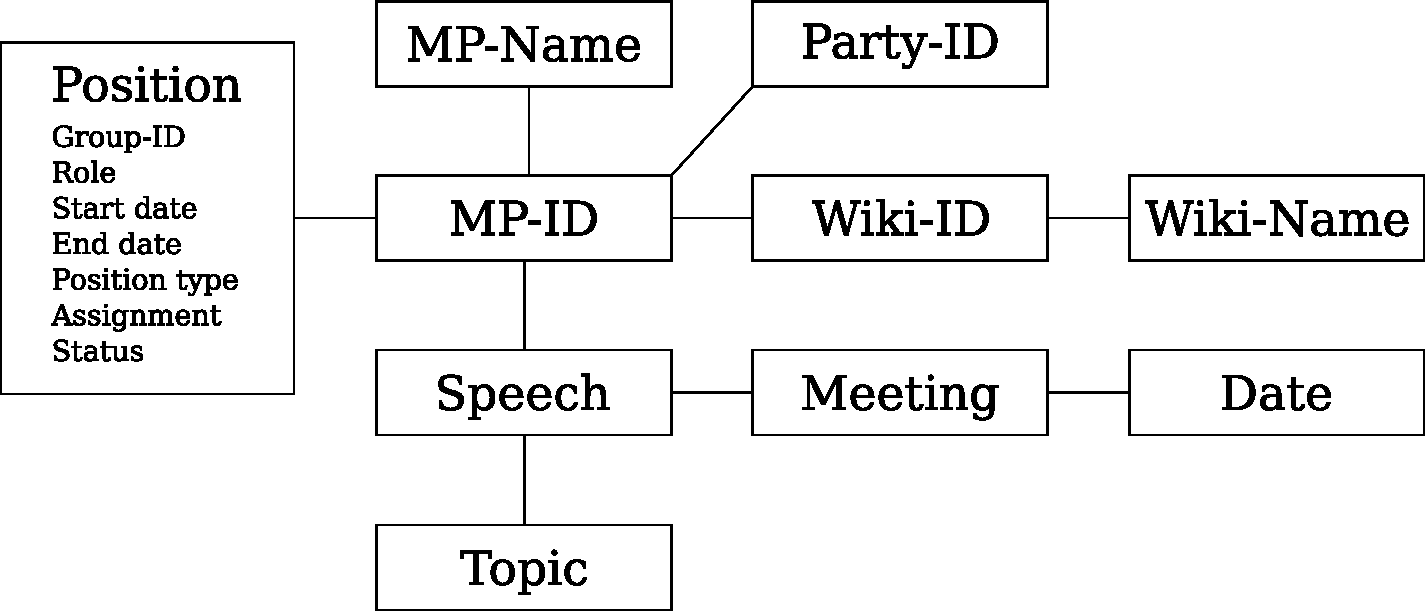
\includegraphics[width=12cm]{images/graph-drawing.pdf}
 \caption{\label{mp-graph} A semantic graph of Swedish MPs and debates.}
\end{figure*}

\subsection{Implementation}

For our rendering of these data as a semantic graph, we chose to create a deductive database in SWI-Prolog, and combine it with the Pengines framework in order to offer web access. Prolog's modular nature allows for very quick prototyping and makes it easy to combine existing rules instead of writing complicated queries such as would be required with SQL or SPARQL. With Pengines, web access is offered simultaneously through a web interface and RPC (Remote Procedure Call) commands passed directly to the server from any Prolog client \cite{lager_pengines_2014}.



Our Prolog database ended up consisting of a number of files, each mapping identifiers and properties to each other. In order to make NER as accurate as possible, we created mappings to MPs' names both as they are listed in the Swedish parliament and how they appear on Wikipedia. This, of course, includes a mapping between unique MP IDs in the parliament and their respective Wikidata-ID, which can potentially be of use for further integration with other analytical tools. For MPs, we also created a file listing their party affiliation that probably will be a necessary step in resolving name ambiguity, as well the previously mentioned position file that details their formal time in parliament and and activity in various commissions. Finally, we have two files that map meetings to dates and debate topics, respectively. An approximation of the resulting graph can be seen in figure \ref{mp-graph}.\footnote{An approximation in the sense that Prolog predicates can have any number of arguments. The Speech and Meeting nodes are for instance mapped to MP-ID and each other in the same predicate.} The edges should be read as \emph{has} or \emph{is}, with either MP-ID or the node closest to it as the subject.

\section{Usage Details}

The Swedish PoliGraph is available to use and download from \url{https://spraakbanken.gu.se/poligraph/} under a Creative Commons Attribution licence.\footnote{\url{https://creativecommons.org/licenses/by/4.0/}} We ask that this paper be cited in any published work using the code or the graph.

\subsection{Rule Construction}

In contrast to relational database queries, Prolog queries are largely dependent on rule construction. For the Swedish PoliGraph, we have created a small set of specialised rules for the purpose of disambiguating names and titles that specifically refer to MPs. A Prolog rule is essentially a list of predicates that must be true in order to satisfy a query. These predicates can be either facts or other rules. Any argument can be substituted with a variable that will, when queried, provide any answer for which that predicate would be true. To give an example, a rule stating that a given politician was an elected and working MP on a given date would be:

\begin{lstlisting}
was_in_rd(Name, Date) :-
    rid_sname(Rid, Name),
    position(Rid,'kam',_,From,Tom,_,_,Status),
    Date >= From,
    Date =< Tom,
    Status \= 'Ledig'.
\end{lstlisting}
%
In somewhat clearer English, this rule states that: A person with a given \emph{Name} was an elected and working MP on a given \emph{Date} \textbf{IF} there exists a mapping from that name to an MP-ID \textbf{AND} that MP-ID had a position in \emph{kam} (eng: the parliament) in that period \textbf{AND} their status in that time was not \emph{Ledig} (eng: away).

\subsection{Using the Swedish PoliGraph}

There are three ways of using the Swedish PoliGraph: (1) local querying with SWI-Prolog; (2) remote querying with SWI-Prolog and Pengines; and (3) via the web interface. Of these, the latter will necessarily be more limited in functionality than the other two, since a practically usable web interface will not be able to reproduce the flexibility that Prolog queries provide.

\begin{table*}[t!]
\fontsize{10pt}{12pt}\selectfont
\begin{center}
\begin{tabular}{|l|l|}
\hline \textbf{Predicate} & \textbf{Description} \\ \hline
\texttt{rid\_sname/2} & Maps an MP-ID to that person's sorting name, e.g. 'Löfven,Stefan' \\
\texttt{rid\_wname/2} & Maps an MP-ID to that person's Wikipedia name, e.g. 'Stefan Löfven' \\
\texttt{rid\_lname/2} & Maps an MP-ID to that person's last name \\
\texttt{rid\_fname/2} & Maps an MP-ID to that person's first name \\
\texttt{rid\_name/2} & Maps an MP-ID to any of the names above \\
\texttt{rid\_wid/2} & Maps an MP-ID to that person's Wikidata-ID \\
\texttt{rid\_party/2} & Maps an MP-ID to that person's party affiliation \\
\texttt{position/8} & See section \ref{sec:mp} for details \\
\texttt{anforande/3} & Maps a speech to a meeting number (dok\_id) and an MP-ID \\
\texttt{dokid\_date/2} & Maps a meeting number (dok\_id) to its date \\
\texttt{meet\_anf\_topic/3} & Maps a topic to a meeting number (dok\_id) and a speech number \\
\texttt{had\_previous\_anf/8} & Matches previous speeches. See section \ref{sec:querying} for details\\
\texttt{had\_anf/6} & Gives speeches with topic, speaker, speech number, 
   party and dok\_id  \\
\texttt{had\_anf/4} & Gives the name, ID and party affiliation for all speeches
   on a given date \\
\texttt{was\_in\_rd/3} & Who was in the parliament in a given period \\
\texttt{was\_mp/3} & Who was an elected MP (non-minister) in a given period \\
\texttt{was\_minister/3} & Who was a minister in a given period \\
\texttt{was\_ledig/3} & Who was on leave from the parliament in a given period \\
\texttt{has\_position/3} & A simplification of position/8 --
   Matches MP's to their assignments \\
\hline
\end{tabular}
\end{center}
\normalfont
\caption{\label{pred-table} A list of currently defined predicates. }
\end{table*}

\subsubsection{Local Querying}
\label{sec:querying}

A central feature of Prolog as a programming language is its \emph{declarative} nature. A Prolog program consists of facts and rules, and are usually interacted with in terms of queries, not unlike relational databases. For the Swedish PoliGraph, we have defined a number of predicates that can be queried directly, although it is also possible for a user to define new predicates extending or combining the existent ones.

In order to start using the Swedish PoliGraph locally, start SWI-Prolog and load the main program file with \texttt{[poligraph].} There you will be able to query both the basic facts and the more complex rules. Note that for any argument, you can use either a quoted string or a number to search for an exact match, or use an upper-case string for a variable. Some simple examples are as follows:

\begin{lstlisting}
/* ID of any MP with last name 'Löfven' */
?- rid_lname(Rid,'Löfven').
Rid = 218878014918.

/*Wikidata-ID for an MP-ID */
?- rid_wid(218878014918, Wid).
Wid = 'Q2740012'.

/* Party affiliation for an MP-ID */
?- rid_parti(218878014918, Party).
Party = 'S'.
\end{lstlisting}
%
%Note here that we have used the term \emph{Rid} to signify an MP's unique ID in the Swedish Parliament, otherwise refered to as MP-ID in this paper.
%, and that we have separate predicates for mapping the MP-ID to last name (\texttt{rid\_lname/2}), first name (\texttt{rid\_fname/2}), sorting name (\texttt{rid\_sname/2}) and Wikidata-name (\texttt{rid\_wname/2}), though they can all be queried simultaneously with \texttt{rid\_name/2}.
The main predicate, however, is constructed for the following purpose: We have a speech, in which a name is mentioned. In order to resolve the name, we wish to see who by that name was talking previously in the same debate. Preferably we know both the meeting number (\emph{dok\_id}) and the topic (\emph{rel\_dok\_id}). As an example, in a debate on 2016-12-12 on the topic of communication infrastructure, MP Teres Lindberg mentioned an Erik Ottoson in her speech, which was the 75th speech in that debate. Querying our program, we get the MP-ID, party affiliation and speech number(s) for that person's earlier participation in the debate: %Kanske du vill skriva att om det bara stått Ottoson så kunde vi fått en lista med alla Ottoson som tidigare pratat i debatten och därmet gjort lite disambiguering direkt? På det viset blir det ännu tydligare vad styrkan och värdet med Poligraph är!


\begin{lstlisting}
?- had_previous_anf('Erik Ottoson', Rid, Anf, Party, 'H401TU1', 'H40944', 75, _).
Rid = 832311880029,
Anf = 74,
Party = 'M' ;
Rid = 832311880029,
Anf = 72,
Party = 'M' ;
\end{lstlisting}
%
In more complex cases, a speaker may not provide the full name of the person they refer to, but rather just their last name or a phrase that only includes their party affiliation. We can then use the same predicate, retrieving the same information plus any additional matches. Where there exists ambiguity in the results, such as several people with the same last name or party affiliation, we can apply simple heuristics, e.g. the last speech before the current speaker's, to identify our target.

In a given query, any of the information we provide can be substituted with a variable, or vice versa. This means that we can get all speeches from a given party in a given debate by using variables for everything except Party and Topic:

\begin{lstlisting}
?- had_anf(Name, Rid, Anf, 'S', 'H401TU1', Meeting).
Name = 'Lindberg',
Rid = 559925283228,
Anf = 73,
Meeting = 'H40944' ;
Name = 'Johansson',
Rid = 691264514114,
Anf = 63,
Meeting = 'H40944' ;
\end{lstlisting}
%
A complete list of currently defined predicates can be seen in table \ref{pred-table}. 

\subsubsection{Remote Querying with Pengines}

By using the Pengines library for SWI-Prolog, the Swedish PoliGraph can be queried remotely. This works essentially the same as local querying, except that the query is wrapped in a predicate \texttt{pengine\_rpc/3}.\footnote{The trailing \texttt{/3} is a Prolog convention to show the arity of a predicate.} The predicate takes three arguments: The URL of the Pengines server, the predicate you wish to run and a list of options, which must include the name of the application on the server. Submitting our previous example over \texttt{pengine\_rpc/3} would look like this:

\begin{lstlisting}
?- pengine_rpc(
  'https://spraakbanken.gu.se/poligraph/',
  rid_lname(Rid,'Löfven'),
  [application(poligraph)]
).
\end{lstlisting}
%
Pengines also allows for several other options, such as specifying which information should be transferred between the client and the server and passing user-created predicates to be used in the query. For details on these options, we refer to Lager and Wielemaker \cite{lager_pengines_2014} and the official Pengines documentation\footnote{\url{http://www.swi-prolog.org/pldoc/package/pengines.html}}.



\subsubsection{The Web Interface}

The web interface is by necessity simplified and only allows for a few selected queries. As such it is primarily intended for demonstration purposes, but it can also be used for qualitative research.



\section{Related Work}

While argumentation mining is a recent field of study where little has been done on parliamentary data (see e.g. \cite{lippi_argumentation_2016} for a good overview), semantic networks are almost as old as computers themselves, starting with a linguistic application by the Cambridge Language Research Unit in 1956 \cite{lehmann_semantic_1992}. An essential part of the semantic web, there now exist large-scale semantic graphs on most subjects, the most comprehensive project being the Wikipedia-sourced DBpedia \cite{lehmann_dbpedia_2015}. For parliamentary data, the situation has improved over the last few years, and with the increasing implementation of public open data policies we can expect to see much further work in that domain. To our knowledge, the largest project for creating a semantic network from parliamentary data was Talk of Europe, which resulted in the LinkedEP Dataset \cite{hollink_talk_2017}, covering all plenary debates held in the European Parliament between July 1999 and July 2017 \cite{van_aggelen_debates_2017}, as well as biographical information about the members of parliament sourced from Høyland et al. \cite{hoyland_forum_2009}. We have also seen this inspire national efforts such as Talk of Norway \cite{lapponi_talk_2018}, while several earlier projects are mentioned by Van Aggelen et al. \cite{van_aggelen_debates_2017}.

\section{Conclusions and Future Work}

We have created the Swedish PoliGraph specifically for named entity resolution and argumentation mining, and hope that it will prove fruitful to that end. Our next step will be NER, and while the current version of the graph is tailored for this, future needs may encourage us to augment it with further metadata, e.g. as additional features to be used in argumentation mining.

We also hope that this graph can be useful outside of our planned scope. The Swedish PoliGraph is both detailed and flexible enough that it can purposefully serve any project dealing with Swedish MPs and debates, be it academic, educational or journalistic.